\documentclass[a4paper,11pt]{article}
\usepackage{amsmath, amssymb, graphicx, siunitx, subcaption, float, booktabs}
\usepackage[margin=1.5cm]{geometry}  % margins set to 1.5 cm
\usepackage{titlesec}
\usepackage{physics}
\usepackage{xcolor}
\usepackage{caption}

\title{\textbf{Branchline Design Using Microstrip Technology}}
\author{Amirkahshayar Maghsoud}
\date{}

\begin{document}

\maketitle
\section{Introduction}

This section presents the data used for the computations:
\[
f_0 = 1290~\text{MHz}, \qquad
k = 4.6, \qquad
Z_0 = 80~\Omega, \qquad
F = 1, \qquad
h = 2.9~\text{mm}, \qquad
\varepsilon_r = 3.5.
\]

\section{$Z_{01}$ and $Z_{02}$ Solutions}

The analysis can be performed using the even- and odd-mode generators, either by exciting ports 1 and 4 or by exciting ports 3 and 4.  
When applying the even- and odd-mode generators to ports 1 and 4, the following ABCD matrix holds:
\[
\mathbf{ABCD} =
\begin{bmatrix}
\pm\dfrac{Z_{02}}{Z_{01}} &
j\,Z_{02} \\[6pt]
j\,Z_{02}\!\left( \dfrac{1}{Z_{02}^{2}} - \dfrac{1}{Z_{01}^{2}} \right) &
\pm\dfrac{Z_{02}}{Z_{01}}
\end{bmatrix}.
\]
The output of the signals at ports is the following:

\begin{figure}[h!]
\[
\begin{minipage}{0.45\textwidth}
\[
\begin{aligned}
b_{4} &= \frac{a_{4}}{2}\,\Gamma_{\text{even}} + \frac{a_{4}}{2}\,\Gamma_{\text{odd}}, \\[4pt]
b_{3} &= \frac{a_{4}}{2}\,T_{\text{even}} + \frac{a_{4}}{2}\,T_{\text{odd}}
\end{aligned}
\]
\end{minipage}
\hfill
\begin{minipage}{0.45\textwidth}
\[
\begin{aligned}
b_{1} &= \frac{a_{4}}{2}\,\Gamma_{\text{even}} - \frac{a_{4}}{2}\,\Gamma_{\text{odd}}, \\[4pt]
b_{2} &= \frac{a_{4}}{2}\,T_{\text{even}} - \frac{a_{4}}{2}\,T_{\text{odd}}
\end{aligned}
\]
\end{minipage}
\]
\end{figure}


From the exercise requirements, the following boundary conditions on the scattering parameters hold:
\[
S_{44} = 0, \qquad S_{41} = 0.
\]

These conditions imply that \(b_1\) and \(b_4\) are zero, as stated by the definition of the scattering parameters.
Additionally, since it is already known that \(a_4 \neq 0\), we obtain the following conditions:
\[
\Gamma_{\text{even}} + \Gamma_{\text{odd}} = 0,
\qquad
\Gamma_{\text{even}} - \Gamma_{\text{odd}} = 0,
\]
which together imply
\[
\Gamma_{\text{even}} = \Gamma_{\text{odd}} = 0.
\]

\subsection*{Reflection coefficients from the ABCD entries}

For a two-port network described by the \(2\times2\) ABCD matrix
\(\begin{bmatrix}A & B\\[2pt] C & D\end{bmatrix}\),
the (normalized) reflection coefficient \(\Gamma\) at the input port may be written in the common form
\[
\Gamma \;=\; \frac{A + B - C - D}{A + B + C + D}.
\]
Applying this to the even and odd matrices resulting in the following  
\[
\Gamma_{\text{even}}
=\frac{A_{e}+B_{e}-C_{e}-D_{e}}{A_{e}+B_{e}+C_{e}+D_{e}},\qquad
\Gamma_{\text{odd}}
=\frac{A_{o}+B_{o}-C_{o}-D_{o}}{A_{o}+B_{o}+C_{o}+D_{o}}.
\]


Computing the common numerator that appears in \(\Gamma\):
\[
A+B-C-D
= jZ_{02}\Big[\,1 -\Big(\dfrac{1}{Z_{02}^{2}}-\dfrac{1}{Z_{01}^{2}}\Big)\Big]
= jZ_{02}\Big(1-\dfrac{1}{Z_{02}^{2}}+\dfrac{1}{Z_{01}^{2}}\Big).
\]

Therefore \(\Gamma_{\text{even}}=0\) (and similarly \(\Gamma_{\text{odd}}=0\)) is achieved if and only if the numerator vanishes:
\[
1-\dfrac{1}{Z_{02}^{2}}+\dfrac{1}{Z_{01}^{2}} = 0
\quad\Longrightarrow\quad
\dfrac{1}{Z_{02}^{2}}-\dfrac{1}{Z_{01}^{2}} = 1.
\]

\[
\boxed{\;\dfrac{1}{Z_{02}^{2}}-\dfrac{1}{Z_{01}^{2}} = 1\; }.
\]

\subsection*{$S$-Parameters}

In an analogous way, since $S_{24} = b_2 / a_4$, we get the following equation:
\[
S_{24} = \frac{T_{\text{even}} - T_{\text{odd}}}{2} = -\sqrt{1 - Z_{02}^{2}}.
\]

And for $S_{34}$:
\[
S_{34} = \frac{T_{\text{even}} + T_{\text{odd}}}{2} = -j Z_{02}^{2}.
\]
And finally the scattering matrix results in
\[
\mathbf{S} =
\begin{bmatrix}
0 & -j\,z_{02} & -\sqrt{1-z_{02}^2} & 0 \\[2mm]
-j\,z_{02} & 0 & 0 & -\sqrt{1-z_{02}^2} \\[1mm]
-\sqrt{1-z_{02}^2} & 0 & 0 & -j\,z_{02} \\[1mm]
0 & -\sqrt{1-z_{02}^2} & -j\,z_{02} & 0
\end{bmatrix}.
\]


The final results for the calculations for the impedances are summarized below:
\[
Z_{01} = 154.4205~\Omega, \qquad
Z_{02} = 71.0335~\Omega,
\]


\section{Hammerstad Approximation}

Under the Hammerstad model, the formulas are valid under the following conditions:
\[
0.05<\frac{w}{h} < 20, \qquad \varepsilon_r < 16.
\]

If the characteristic impedance \( Z_c \) and the relative permittivity \( \varepsilon_r \) are known quantities, then the following relations hold for the effective permittivity and characteristic parameters of the microstrip line.
The characteristic factor $A$ is given by
\[
A = \frac{Z}{60}\,\sqrt{\frac{\varepsilon_r + 1}{2}} 
      + \frac{\varepsilon_r - 1}{\varepsilon_r + 1} 
        \left(0.23 + \frac{0.11}{\varepsilon_r}\right),
\]


The width-to-height ratio of the microstrip is given by
\[
\frac{w}{h} = \frac{8}{\exp(A) - 2\,\exp(-A)},
\]
and must satisfy the condition
\[
\frac{w}{h} < 2.
\]

so the actual microstrip width is
\[
w = \left(\frac{w}{h}\right) h.
\]

The effective dielectric constant in case of $w/h > 1$, which is the case for $Z_{02}$, is 
\[
\varepsilon_{\text{eff}} = \frac{\varepsilon_r + 1}{2} 
+ \frac{\varepsilon_r - 1}{2} 
\left( 1 + \frac{12\,h}{w} \right)^{-1/2}.
\] 

And for $Z_{01}$ and $Z_0$ where $w/h < 1$,
\[
\varepsilon_{\text{eff}} = \frac{\varepsilon_r + 1}{2} 
+ \frac{\varepsilon_r - 1}{2} \left[ 
\left( 1 + \frac{12\,h}{w} \right)^{-1/2} 
+ 0.04 \left( 1 - \frac{w}{h} \right)^2 
\right].
\]
\begin{table}[h!]
\centering
\begin{tabular}{lcccc}
\toprule
\textbf{Line} & \textbf{$A$} & \textbf{$w/h$} & \textbf{$h$ [mm]} & \textbf{$\varepsilon_{\text{eff}}$} \\
\midrule
Ports & 2.14 & 0.9627 & 2.9 &  2.59 \\
Horizontal branch line ($Z_{01}$) & 4.0058 & 0.1458 & 2.9 & 2.4526\\
Vertical branch line ($Z_{02}$) & 1.9211 & 1.2244 & 2.9 & 2.6303 \\
\bottomrule
\end{tabular}
\caption{Hammerstad formula results for microstrip line sections, including effective dielectric constants.}
\end{table}



The guided wavelength is
\[
\lambda = \frac{c}{f_0 \sqrt{\varepsilon_{\text{eff}}}},
\]

and the quarter-wavelength line length for the horizontal and vertical parts of the branchline is given with the following formula, and the results are summarized in the table below:
\[
l = \frac{\lambda}{4}.
\]




\begin{table}[h!]
\centering
\begin{tabular}{lccc}
\toprule
\textbf{Line} & \textbf{Impedance $Z_0$ [\(\Omega\)]} & \textbf{Width $W$ [mm]} & \textbf{Length $l$ [m]} \\
\midrule
Ports & 80 & -- & -- \\
Horizontal branch line ($Z_{01}$) & 154.42 & 0.4228 & 0.0371 \\
Vertical branch line ($Z_{02}$) & 71.03 & 3.5499 & 0.0358 \\
\bottomrule
\end{tabular}
\caption{Summary of microstrip line dimensions using Hammerstad's approximation.}
\end{table}




\section{Scattering Parameters}

The scattering parameters have been obtained using \textsc{MATLAB} by defining the impedances 
\( Z_{01} \) and \( Z_{02} \), and characterizing the device using the total ABCD matrix for the 
even and odd modes. Using these matrices, the transmission and reflection coefficients were 
computed to derive the scattering parameters, following the same procedure described in 
Section~2. The resulting values are presented below.

\vspace{1cm}
\begin{figure}[h!]
\centering

\begin{subfigure}[b]{0.48\textwidth}
    \centering
    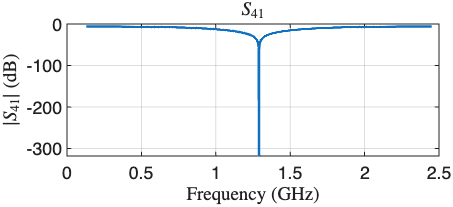
\includegraphics[width=\textwidth]{s41mat.png}
    \caption{$S_{41}$}
    \label{fig:s41}
\end{subfigure}
\hfill
\begin{subfigure}[b]{0.48\textwidth}
    \centering
    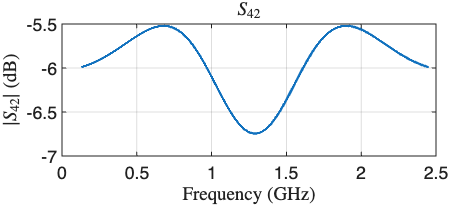
\includegraphics[width=\textwidth]{s42mat.png}
    \caption{$S_{42}$}
    \label{fig:s42}
\end{subfigure}


\label{fig:main}
\end{figure}

\begin{figure}[h!]
\centering
\vspace{0.5cm}

\begin{subfigure}[b]{0.48\textwidth}
    \centering
    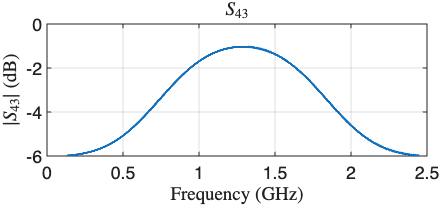
\includegraphics[width=\textwidth]{s43mat.png}
    \caption{$S_{43}$}
    \label{fig:s43}
\end{subfigure}
\hfill
\begin{subfigure}[b]{0.48\textwidth}
    \centering
    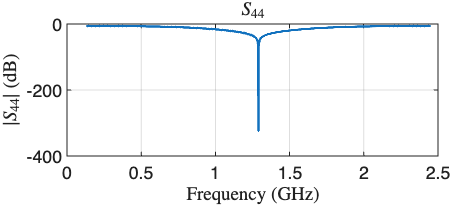
\includegraphics[width=\textwidth]{s44mat.png}
    \caption{$S_{44}$}
    \label{fig:s44}
\end{subfigure}

\caption{Scattering parameter results from MATLAB.}
\label{fig:main}
\end{figure}
\vspace{5cm}

\section{Scattering Parameters with $\pm 5\%$ Variation of $Z_{01}$ and $Z_{02}$}

Using a random variation of $\pm 5\%$ and a random ensemble of 20 samples, the following results are obtained:
\begin{figure}[h!]
\centering

\begin{subfigure}[b]{0.45\textwidth}
    \centering
    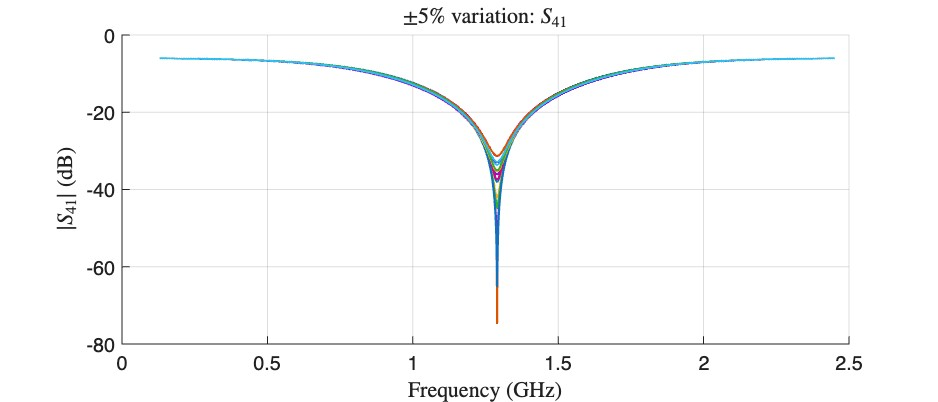
\includegraphics[width=\textwidth]{s41.jpg}
    \caption{S\textsubscript{41}}
    \label{fig:sub1}
\end{subfigure}
\hfill
\begin{subfigure}[b]{0.45\textwidth}
    \centering
    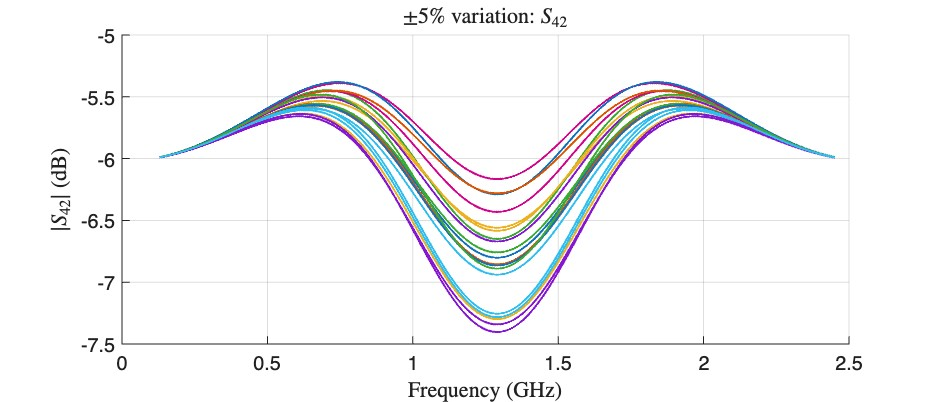
\includegraphics[width=\textwidth]{s42.jpg}
    \caption{S\textsubscript{42}}
    \label{fig:sub2}
\end{subfigure}

\vspace{0.5cm}

\begin{subfigure}[b]{0.45\textwidth}
    \centering
    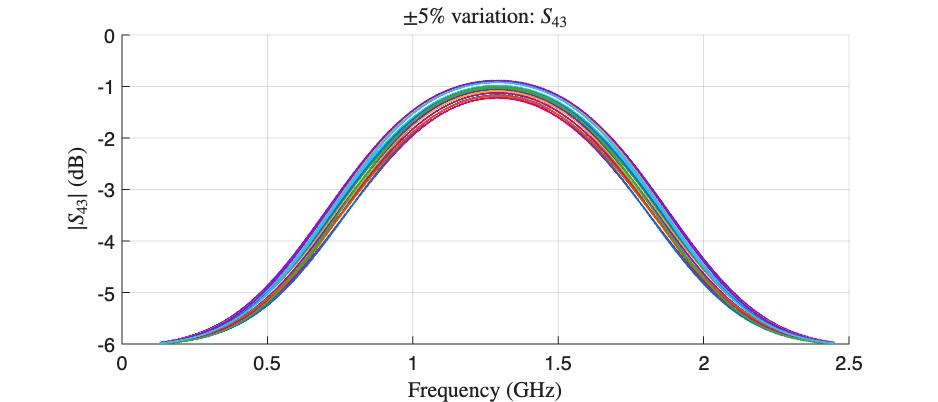
\includegraphics[width=\textwidth]{s43.jpg}
    \caption{S\textsubscript{43}}
    \label{fig:sub3}
\end{subfigure}
\hfill
\begin{subfigure}[b]{0.45\textwidth}
    \centering
    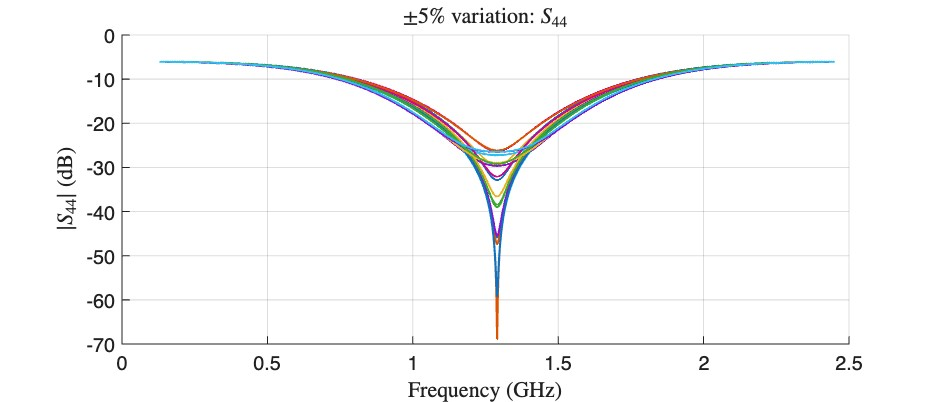
\includegraphics[width=\textwidth]{s44.jpg}
    \caption{S\textsubscript{44}}
    \label{fig:sub4}
\end{subfigure}

\caption{Scattering parameters $S_{41}$ to $S_{44}$ with $\pm 5\%$ variation.}
\label{fig:main}
\end{figure}

\section{CST Simulation}

For the CST simulation, the following data have been used: 
\( h = 2.9 \), \( \varepsilon_r = 3.5 \), and \( k = 7 \).
Additionally, the substrate has been realized using loss-free FR-4, with the dielectric constant adjusted to 
\( \varepsilon_r = 3.5 \) in order to match the exercise specifications.

\begin{table}[h!]
\centering
\begin{tabular}{lccc}
\toprule
\textbf{Line} & \textbf{Impedance $Z_0$ [\(\Omega\)]} & \textbf{Width $W$ [mm]} & \textbf{Length $l$ [m]} \\
\midrule
Ports & 80 & 2.7918 & -- \\
Horizontal branch line ($Z_{01}$) & 81.6363 & 2.6754 & 36.2 \\
Vertical branch line ($Z_{02}$) & 57.1314 & 5.2620 & 36.4 \\
\bottomrule
\end{tabular}
\caption{Summary of microstrip line dimensions for CST simulation}
\end{table}
\begin{figure}[h!]
\centering

\begin{subfigure}[b]{0.45\textwidth}
    \centering
    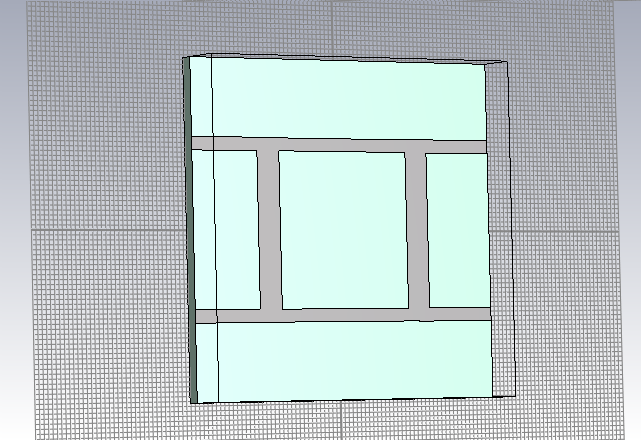
\includegraphics[width=\textwidth]{3D_2.png}
    \caption{Branchline using microstrip technology}
    \label{fig:sub4}
\end{subfigure}


\label{fig:main}
\end{figure}



\begin{figure}[h!]
\centering

% --- Row 1 ---
\begin{subfigure}[b]{0.45\textwidth}
    \centering
    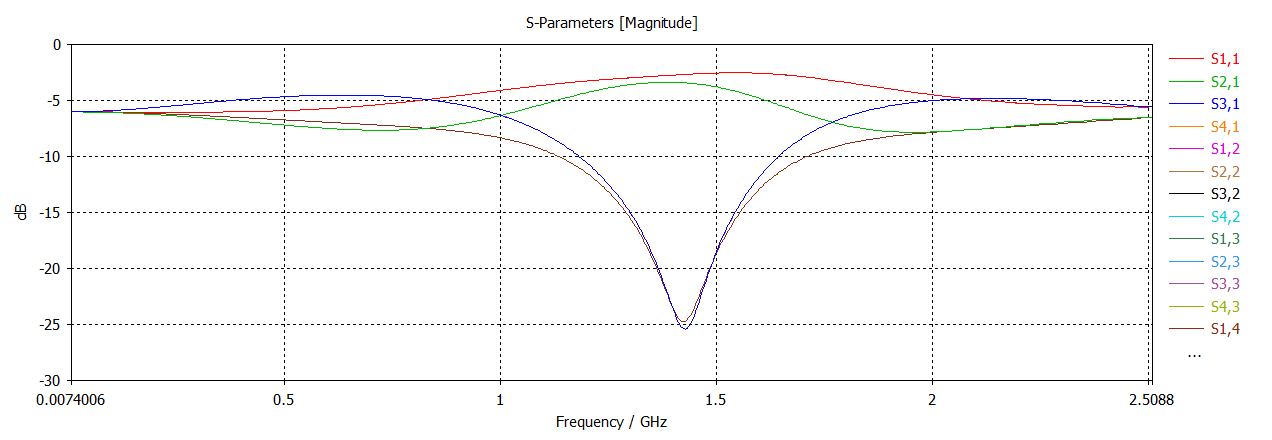
\includegraphics[width=\textwidth]{S-Parameters.png}
    \caption{S Parameters using CST}
    \label{fig:sparams}
\end{subfigure}
\hfill
\begin{subfigure}[b]{0.45\textwidth}
    \centering
    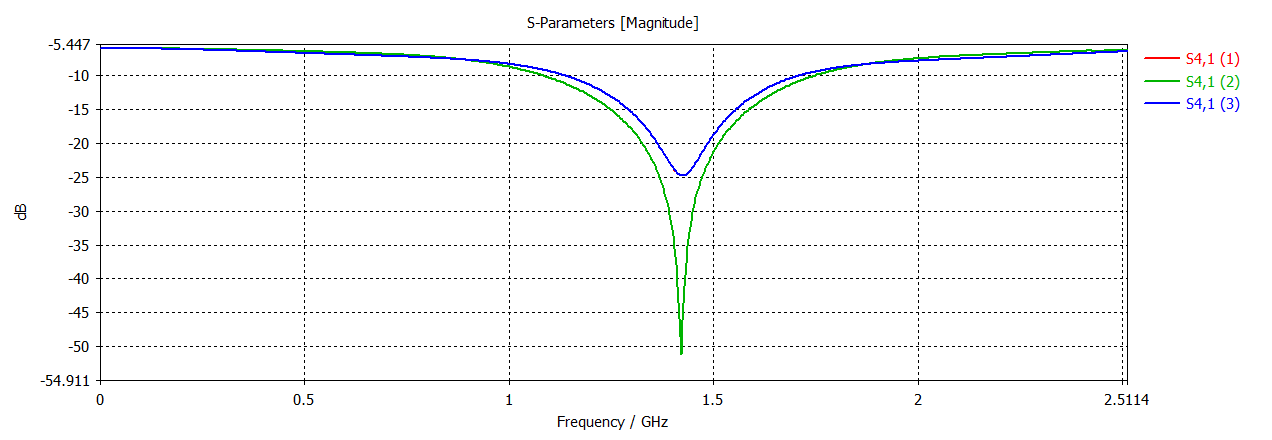
\includegraphics[width=\textwidth]{S4,1.png}
    \caption{S\textsubscript{41}}
    \label{fig:s41}
\end{subfigure}

\vspace{0.5cm}

% --- Row 2 ---
\begin{subfigure}[b]{0.45\textwidth}
    \centering
    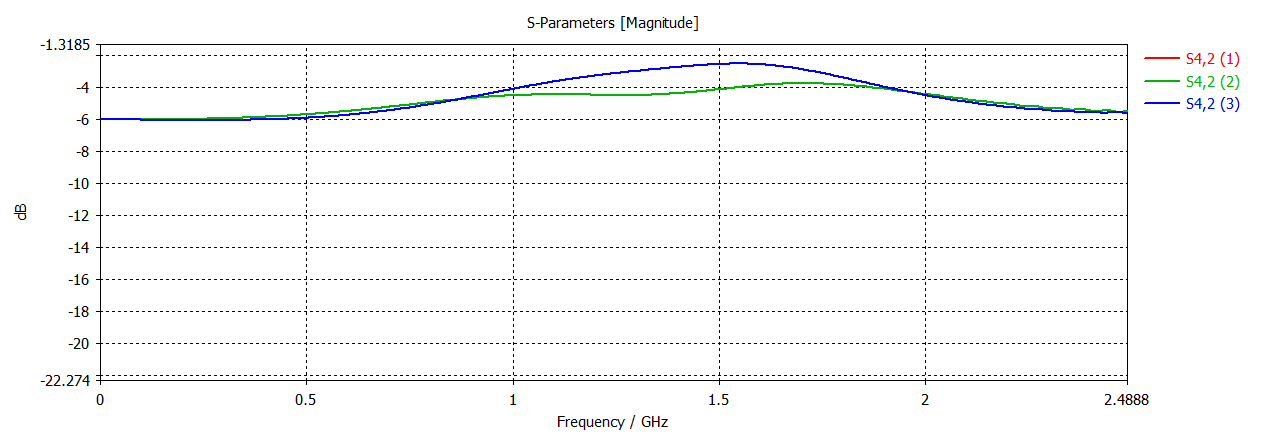
\includegraphics[width=\textwidth]{S4,2.png}
    \caption{S\textsubscript{42}}
    \label{fig:s42}
\end{subfigure}
\hfill
\begin{subfigure}[b]{0.45\textwidth}
    \centering
    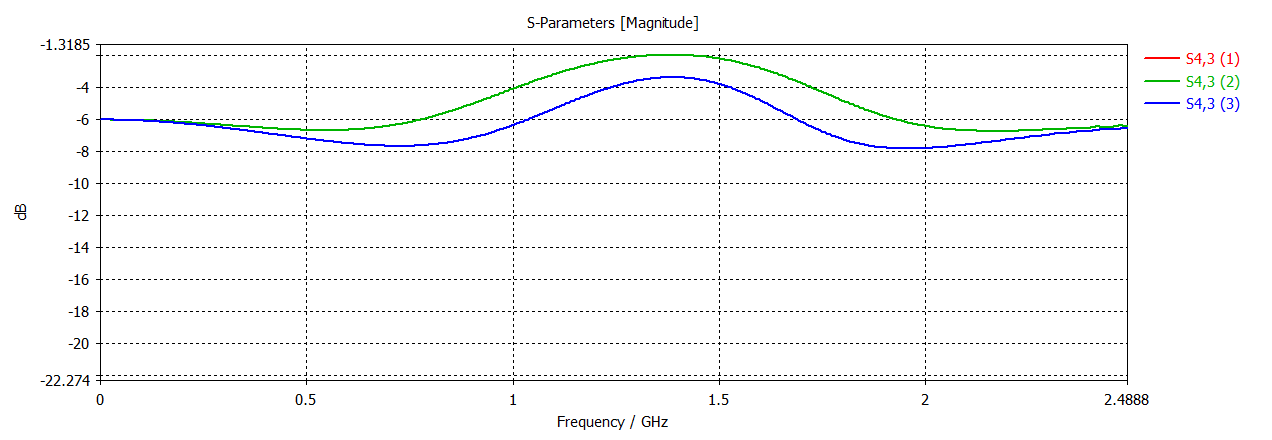
\includegraphics[width=\textwidth]{S4,3.png}
    \caption{S\textsubscript{43}}
    \label{fig:s43}
\end{subfigure}

\vspace{0.5cm}

% --- Last image centered ---
\begin{subfigure}[b]{0.45\textwidth}
    \centering
    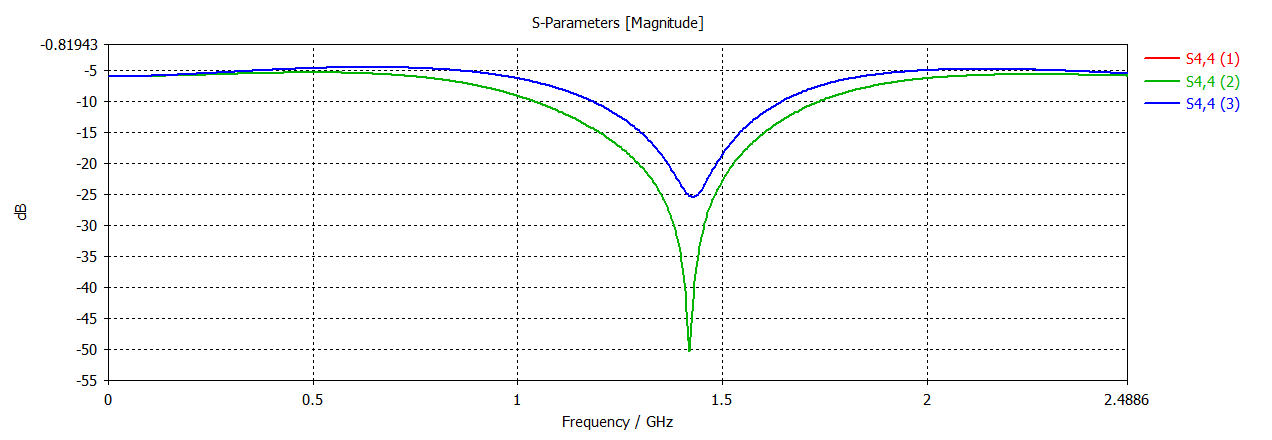
\includegraphics[width=\textwidth]{S4,4.png}
    \caption{S\textsubscript{44}}
    \label{fig:s44}
\end{subfigure}

\caption{Scattering parameters $S_{41}$ to $S_{44}$ using CST}
\label{fig:main}
\end{figure}

Additionally, checking the results of the CST simulation with \textsc{MATLAB} shows that they agree well. 
For completeness, the corresponding \textsc{MATLAB} results will be presented below, using the same parameters as before.
\begin{figure}[H]
\centering

% --- Row 1 ---
\begin{subfigure}[b]{0.4\textwidth}
    \centering
    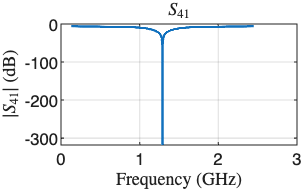
\includegraphics[width=\textwidth]{s41k7.png}
    \caption{S\textsubscript{41} (k = 7)}
    \label{fig:s41}
\end{subfigure}
\hfill
\begin{subfigure}[b]{0.4\textwidth}
    \centering
    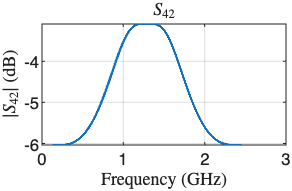
\includegraphics[width=\textwidth]{s42k7.png}
    \caption{S\textsubscript{42} (k = 7)}
    \label{fig:s42}
\end{subfigure}

\vspace{0.6cm}

\caption{Scattering parameters obtained from \textsc{MATLAB} for $k = 7$.}
\label{fig:sparams}
\end{figure}

\vspace{3cm}

\begin{figure}[H]
\centering

% --- Row 2 ---
\begin{subfigure}[b]{0.45\textwidth}
    \centering
    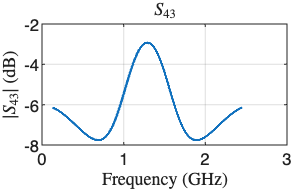
\includegraphics[width=\textwidth]{s43k7.png}
    \caption{S\textsubscript{43} (k = 7)}
    \label{fig:s43}
\end{subfigure}
\hfill
\begin{subfigure}[b]{0.45\textwidth}
    \centering
    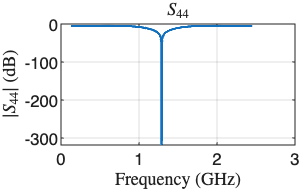
\includegraphics[width=\textwidth]{s44k7.png}
    \caption{S\textsubscript{44} (k = 7)}
    \label{fig:s44}
\end{subfigure}

\caption{Scattering parameters obtained from \textsc{MATLAB} for $k = 7$.}
\label{fig:sparams}
\end{figure}





\end{document}
